\documentclass[10pt, a4paper]{article}
\usepackage[top=3cm, bottom=4cm, left=3.5cm, right=3.5cm]{geometry}
\usepackage{amsmath,amsthm,amsfonts,amssymb,amscd, fancyhdr, color, comment, graphicx, environ, pifont, blkarray}
\usepackage{float}
\usepackage{mathrsfs}
\usepackage[framemethod=TikZ]{mdframed}
\usepackage{enumerate}
\usepackage[shortlabels]{enumitem}
\usepackage{fancyhdr}
\usepackage{indentfirst}
\usepackage{listings}
\usepackage{sectsty}
\usepackage{thmtools}
\usepackage{shadethm}
\usepackage{hyperref}
\usepackage{setspace}
\usepackage[linguistics]{forest}
\allowdisplaybreaks[4]
\hypersetup{
    colorlinks=true,
    linkcolor=blue,
    filecolor=magenta,      
    urlcolor=blue,
}
\mdfsetup{skipabove=\topskip,skipbelow=\topskip}
\mdfdefinestyle{theoremstyle}{%
linecolor=black,linewidth=1pt,%
frametitlerule=true,%
frametitlebackgroundcolor=gray!20,
innertopmargin=\topskip,
}
\mdtheorem[style=theoremstyle]{Problem}{Problem}
\newenvironment{Solution}{\textbf{Solution.}}

\definecolor{codegreen}{rgb}{0,0.6,0}
\definecolor{codegray}{rgb}{0.5,0.5,0.5}
\definecolor{codepurple}{rgb}{0.58,0,0.82}
\definecolor{backcolour}{rgb}{0.95,0.95,0.92}

\lstdefinestyle{mystyle}{
    backgroundcolor=\color{backcolour},   
    commentstyle=\color{codegreen},
    keywordstyle=\color{magenta},
    numberstyle=\tiny\color{codegray},
    stringstyle=\color{codepurple},
    basicstyle=\ttfamily\footnotesize,
    breakatwhitespace=false,         
    breaklines=true,                 
    captionpos=b,                    
    keepspaces=true,                 
    numbers=left,                    
    numbersep=5pt,                  
    showspaces=false,                
    showstringspaces=false,
    showtabs=false,                  
    tabsize=2
}

\lstset{style=mystyle}
\newcommand{\norm}[1]{\left\lVert#1\right\rVert}     
\newcommand\course{Introduction to Applied Mathematics}                          
\newcommand\hwnumber{MATH40007}                                                
\pagestyle{fancy}
\headheight 35pt
\lhead{\today}
\rhead{
\includegraphics[width=2.5cm]{icl_logo.png}}
\lfoot{}
\pagenumbering{arabic}
\cfoot{\small\thepage}
\rfoot{}
\headsep 1.2em
\renewcommand{\baselinestretch}{1.25}
\renewcommand{\labelenumi}{\alph{enumi})}
\newcommand{\Z}{\mathbb Z}
\newcommand{\R}{\mathbb R}
\newcommand{\Q}{\mathbb Q}
\newcommand{\NN}{\mathbb N}
\newcommand{\PP}{\mathbb P}
\DeclareMathOperator{\Mod}{Mod} 
\renewcommand\lstlistingname{Algorithm}
\renewcommand\lstlistlistingname{Algorithms}
\def\lstlistingautorefname{Alg.}
\newtheorem*{theorem}{Theorem}
\newtheorem*{lemma}{Lemma}
\newtheorem{case}{Case}
\newcommand{\assign}{:=}
\newcommand{\infixiff}{\text{ iff }}
\newcommand{\nobracket}{}
\newcommand{\backassign}{=:}
\newcommand{\tmmathbf}[1]{\ensuremath{\boldsymbol{#1}}}
\newcommand{\tmop}[1]{\ensuremath{\operatorname{#1}}}
\newcommand{\tmtextbf}[1]{\text{{\bfseries{#1}}}}
\newcommand{\tmtextit}[1]{\text{{\itshape{#1}}}}

\newenvironment{itemizedot}{\begin{itemize} \renewcommand{\labelitemi}{$\bullet$}\renewcommand{\labelitemii}{$\bullet$}\renewcommand{\labelitemiii}{$\bullet$}\renewcommand{\labelitemiv}{$\bullet$}}{\end{itemize}}
\catcode`\<=\active \def<{
\fontencoding{T1}\selectfont\symbol{60}\fontencoding{\encodingdefault}}
\catcode`\>=\active \def>{
\fontencoding{T1}\selectfont\symbol{62}\fontencoding{\encodingdefault}}
\catcode`\<=\active \def<{
\fontencoding{T1}\selectfont\symbol{60}\fontencoding{\encodingdefault}}
\begin{document}

\begin{titlepage}
    \begin{center}
        \vspace*{3cm}
            
        \Huge
        \textbf{
        Coursework II}
            
            
        \vspace{1.5cm}
        \Large
            
        \textbf{
        CID number: Trust me, you don't want to know it.}% <-- author
        
            
        \vfill
        
    MATH40007: Introduction to Applied Mathematics , 2023
        \vspace{1cm}
            
        
\includegraphics[width=0.4\textwidth]{icl_logo.png}
        \\
        
        \Large
        
        \today
            
    \end{center}
\end{titlepage}


\newpage
\begin{Problem}
Part I: For any integer $n \geq 0$ define

$$
I_{+}(n) \equiv \int_{0}^{1} e^{y} \sin (n \pi y) d y, \quad I_{-}(n) \equiv \int_{0}^{1} e^{-y} \sin (n \pi y) d y .
$$

(i) Calculate these two integrals explicitly.

(ii) Use the result of part (i) to find the Fourier sine series of both $\sinh y$ and cosh $y$ over the interval $[0,1]$ (you should use ideas from the "Calculus and Applications" course).

Part II: Consider the electric circuit shown in the Figure where the vertical edges have conductance $c$ and the horizontal edges have conductance $d$. Node $2 \mathrm{~N}+1$ is set to unit voltage, while nodes 0 and $\mathrm{N}+1$ to $2 \mathrm{~N}$ are grounded (set to zero voltage). Kirchhoff's current law holds at nodes 1 to $\mathrm{N}$. Let $\hat{\mathbf{x}}$ denote the voltages at nodes 1 to $\mathrm{N}$. The nodes should be ordered as follows: $1,2, \ldots, 2 \mathrm{~N}-1,2 \mathrm{~N}$, $0,2 \mathrm{~N}+1$.

(a) Show that the conductance-weighted Laplacian matrix is

$$
\mathbf{K}=\left(\begin{array}{ccc}
c \mathbf{K}_{N}+d \mathbf{I}_{N} & -d \mathbf{I}_{N} & -c \mathbf{P} \\
-d \mathbf{I}_{N} & d \mathbf{I}_{N} & \mathbf{0} \\
-c \mathbf{P}^{T} & \mathbf{0} & c \mathbf{I}_{2}
\end{array}\right),
$$

where $\mathbf{I}_{j}$ denotes the $j$-by- $j$ identity matrix and $\mathbf{K}_{N}$ is the $N$-by- $N$ matrix familiar from lectures. You should find the $N$-by-2 matrix $\mathbf{P}$.

(b) Let $\left\{\boldsymbol{\Phi}_{\mathbf{j}} \mid j=1, \ldots, N\right\}$ and $\left\{\lambda_{j} \mid j=1, \ldots, N\right\}$ denote the orthonormal eigenvectors and corresponding eigenvalues of $\mathbf{K}_{N}$. By writing

$$
\hat{\mathbf{x}}=\sum_{j=1}^{N} a_{j}(\mu) \boldsymbol{\Phi}_{j}, \quad \mu=\frac{d}{c}
$$

find the coefficients $\left\{a_{j}(\mu) \mid j=1, \ldots, N\right\}$.

\begin{center}
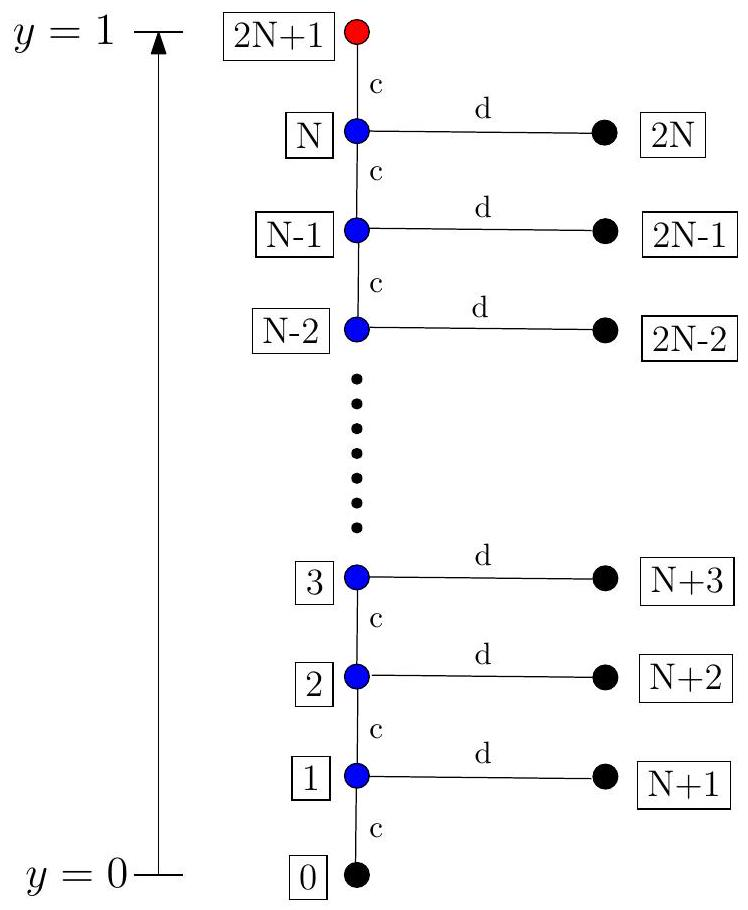
\includegraphics[scale=0.15]{2023_03_08_5758588d6e703b32009fg-2.jpg}
\end{center}

(c) Show that the $n$-th element of $\hat{\mathbf{x}}$ can also be written as

$$
\frac{\lambda_{+}(\mu)^{n}-\lambda_{-}(\mu)^{n}}{\lambda_{+}(\mu)^{N+1}-\lambda_{-}(\mu)^{N+1}}, \quad n=1, \ldots, N,
$$

for suitable choices of the parameters $\lambda_{ \pm}(\mu)$.

(d) The uniqueness theorem for harmonic potentials discussed in lectures has an analogous version when the conductances are not all equal. Use this fact to establish a discrete identity involving your answers to parts (b) and (c).

(e) Now pick $\mu$ to be given by

$$
\mu=\frac{1}{(N+1)^{2}}
$$

and introduce the new variable

$$
y=\frac{n}{(N+1)}
$$

Find the limit of both left- and right-hand sides of the discrete identity you found in part (d) as $N \rightarrow \infty$ with $y$ taken to be fixed.
\end{Problem}
\begin{Solution}
    \begin{itemize}
        \item[\textbf{Part I}:] 
        \begin{itemize}
            \item[(i)] 
            \begin{align*}
                I_+(n) & = \int_0^1 e^y \sin(n \pi y) dy \\
                       & = \int_0^1 sin(n \pi y) d(e^y) \\
                       & = \sin(n \pi y)e^y \bigg|_0^1 -n\pi \int_0^1 e^y \cos(n \pi y) dy \\
                       & = -n\pi \int_0^1 e^y \cos(n \pi y) dy \\
                       & = -n\pi \int_0^1 \cos(n \pi y) d(e^y ) \\
                       & = -n\pi \cos(n \pi y) e^y \bigg|_0^1 - n^2 \pi^2 \int_0^1 e^y \sin(n \pi y) dy \\
                       & = -n\pi (\cos(n \pi) e - 1)  - n^2 \pi^2 I_+(n) \\
                (n^2\pi^2+1) I_+(n) & = n \pi(1-(-1)^n e) \\ 
                I_+(n) & = \frac{n \pi(1-(-1)^n e)}{n^2\pi^2+1} \\
                I_-(n) & = \int_0^1 e^{-y} \sin(n \pi y) dy \\
                       & = - \int_0^1 \sin(n \pi y) d(e^{-y}) \\
                       & = - e^{-y} \sin(n \pi y) \bigg|_0^1 + n\pi \int_0^1 e^{-y} \cos(n \pi y) dy \\
                       & = -n \pi \int_0^1 \cos(n \pi y) d(e^{-y}) \\
                       & = -n \pi \cos(n \pi y) e^{-y} \bigg|_0^1 - n^2 \pi^2 \int_0^1 e^{-y} \sin(n \pi y) dy \\
                       & = -n \pi (\cos(n \pi) e^{-1}-1) - n^2 \pi^2 I_-(n) \\
                I_-(n) + n^2 \pi^2 I_-(n) & = n \pi (1 - (-1)^n e^{-1}) \\
                I_-(n) & = \frac{n \pi (1 - (-1)^n e^{-1})}{n^2 \pi^2 + 1} \\
            \end{align*}
            As conclusion, we have
            \begin{align*}
                I_+(n) & = \frac{n \pi(1-(-1)^n e)}{n^2\pi^2+1}\\
                I_-(n) & = \frac{n \pi (1 - (-1)^n e^{-1})}{n^2 \pi^2 + 1}
            \end{align*}
            \item[(ii)] As $ \sinh y $ is an odd function, we have $a_n = 0$ for all $n$. Therefore, at the interval $[0,1]$, we have
                        \begin{align*}
                            b_n & = 2 \int_0^1 \frac{e^y-e^{-y}}{2} \sin(n \pi y) dy \\
                                & = \int e^y \sin(n \pi y) dy - \int_0^1 e^{-y} \sin(n \pi y) dy\\
                                & = I_+(n) - I_-(n) 
                        \end{align*}
            Hence, the Fourier sine series of $\sinh y$ is
                        \begin{equation*}
                            \sinh y = \sum_{n=1}^{\infty} b_n \sin(n \pi y) = \sum_{n=1}^{\infty} (I_+(n) - I_-(n)) \sin(n \pi y)= \sum_{n=1}^{\infty} \frac{n \pi (-1)^n (e^{-1}-e)}{n^2 \pi + 1} \sin(n \pi y)
                        \end{equation*}
                        For $\cosh y$, it is an even function. We can do the odd extension of $\cosh y$ to get the Fourier sine series of $\cosh y$. Hence,
                        \begin{align*}
                            b_n &= 2 \int_0^1 \frac{e^y+e^{-y}}{2} \sin(n \pi y) dy \\
                                &= \int_0^1 e^y \sin(n \pi y) dy + \int_0^1 e^{-y} \sin(n \pi y) dy \\
                                &= I_+(n) + I_-(n) 
                        \end{align*}
            Hence, the Fourier sine series of $\cosh y$ is
                        \begin{equation*}
                            \cosh y = \sum_{n=1}^{\infty} b_n \sin(n \pi y) = \sum_{n=1}^{\infty} (I_+(n) + I_-(n)) \sin(n \pi y) = \sum_{n=1}^{n} \frac{2 n \pi (-1)^n (e^{-1}+e)}{n^2 \pi + 1} \sin(n \pi y)
                        \end{equation*}
            As conclusion, we have
                        \begin{align*}
                            \sinh y &= \sum_{n=1}^{\infty} \frac{n \pi (-1)^n (e^{-1}-e)}{n^2 \pi + 1} \sin(n \pi y)\\
                            \cosh y &=  \sum_{n=1}^{n} \frac{2 n \pi (-1)^n (e^{-1}+e)}{n^2 \pi + 1} \sin(n \pi y)
                        \end{align*}
            \end{itemize}
        \item[\textbf{Part II}:]
            \begin{itemize}
                \item[(a)] By the order given, The conductance-weighted Laplacian matrix of the graph is given by
                \begin{center}
                    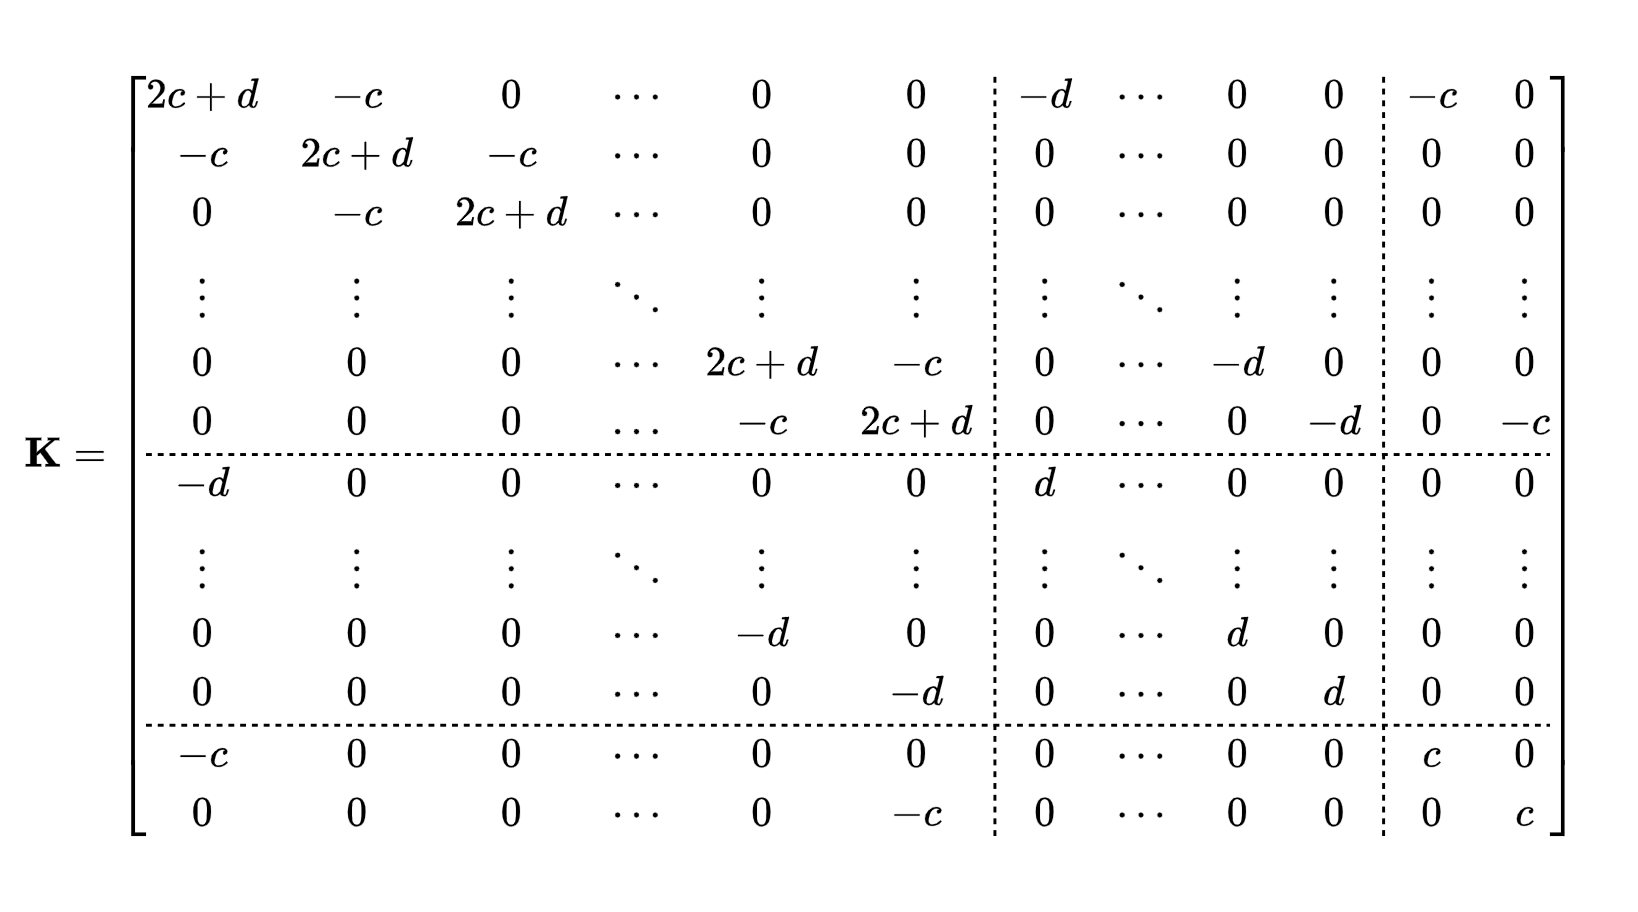
\includegraphics[scale=0.40]{截屏2023-03-13 06.49.19.png}
                \end{center}
                which is equal to
                $$
                \mathbf{K}=\begin{bmatrix}
                c \mathbf{K}_{N}+d \mathbf{I}_{N} & -d \mathbf{I}_{N} & -c \mathbf{P} \\
                -d \mathbf{I}_{N} & d \mathbf{I}_{N} & \mathbf{0} \\
                -c \mathbf{P}^{T} & \mathbf{0} & c \mathbf{I}_{2}
                \end{bmatrix},
                $$
                where $\mathbf{I}_{j}$ denotes the $j$-by- $j$ identity matrix and $\mathbf{K}_{N}$ is the $N$-by- $N$ matrix familiar from lectures and the $N$-by-$N$ matrix $\mathbf{P}$ is given by
                $$\mathbf{P}=\begin{bmatrix}
                    1 &0 \\
                    0 &0\\
                    0 &0 \\
                    \vdots &\vdots \\
                    0 &0 \\
                    0 &1
                \end{bmatrix}               
                    $$
                \item[(b)] For this electric circuit, we have:
                \begin{align}
                \mathbf{K X}&=\mathbf{f}\\
                \begin{bmatrix}
                c \mathbf{K}_{N}+d \mathbf{I}_{N} & -d \mathbf{I}_{N} & -c \mathbf{P} \\
                -d \mathbf{I}_{N} & d \mathbf{I}_{N} & \mathbf{0} \\
                -c \mathbf{P}^{T} & \mathbf{0} & c \mathbf{I}_{2}
                \end{bmatrix}
                \begin{bmatrix}
                    \hat{\mathbf{x}}\\
                    \mathbf{0}\\
                    \hat{\mathbf{e}}
                \end{bmatrix}&=
                \begin{bmatrix}
                    \mathbf{0}\\
                    \mathbf{C_{eff}}\\
                    \hat{\mathbf{f}}
                \end{bmatrix}
                \end{align}
                where $\hat{\mathbf{x}}$ is the vector of the voltages at the nodes $1$ to $N$. Since the nodes at $N+1$ to $2N$ are grounded, the voltages there are all $0$ and $\hat{\mathbf{e}}$ is the vector of the voltages at the voltage source $2N+1$ and $0$, $\mathbf{C_{eff}}$ is the vector of the effective conductance, and $\hat{\mathbf{f}}$ is the vector of the applied voltages. As KCL holds at nodes $1$ to $N$, the flux of nodes $1$ to $N$ are all zero. In ditails, we have
                \begin{equation*}
                    \hat{\mathbf{e}}=\begin{bmatrix}
                        0\\
                        1
                    \end{bmatrix}\;
                \hat{\mathbf{f}}=
                \begin{bmatrix}
                    -f_0\\
                    f_0
                \end{bmatrix}
                \end{equation*}
                The linear system $(2)$ is equivalent to 
                \begin{align}
                    c \mathbf{K}_{N} \hat{\mathbf{x}}+d \mathbf{I}_{N} \hat{\mathbf{x}}-d \mathbf{I}_{N} \mathbf{0} -c \mathbf{P} \hat{\mathbf{e}}&=\mathbf{0}\\
                    d \mathbf{I}_{N} \hat{\mathbf{x}}-d \mathbf{I}_{N} \mathbf{0} & = \mathbf{C_{eff}}\\
                    -c \mathbf{P}^{T} \hat{\mathbf{e}} & = \hat{\mathbf{f}}
                \end{align}
                Let's consider equation $(3)$, it impies that
                \begin{align}
                    c\mathbf{K}_{N} \hat{\mathbf{x}}+d \mathbf{I}_{N} \hat{\mathbf{x}}&=c \mathbf{P} \hat{\mathbf{e}}\\
                    c\mathbf{K}_{N} \hat{\mathbf{x}}+ d \hat{\mathbf{x}}&=c \mathbf{P} \hat{\mathbf{e}}=\begin{bmatrix}
                        0\\
                        0\\
                        \vdots\\
                        c
                    \end{bmatrix}
                \end{align}
                Let us solve equation $(7)$ using the eigenvectors of $\mathbf{K}_N$, which we learnt in the lecture.
                \begin{equation}
                    \mathbf{K}_N \boldsymbol{\Phi}_{j}=\lambda \boldsymbol{\Phi}_{j}, \; j = 1,2,\cdots,N
                \end{equation}
                where

                $$
                \boldsymbol{\Phi}_{j}=\sqrt{\frac{2}{N+1}}\left(\begin{array}{c}
                \sin \left(\frac{j \pi}{N+1}\right) \\
                \sin \left(\frac{2 j \pi}{N+1}\right) \\
                \cdot \\
                \cdot \\
                \sin \left(\frac{n j \pi}{N+1}\right)
                \end{array}\right), \quad j=1, \ldots, N
                $$
                
                which has corresponding eigenvalue
                
                $$
                \lambda_{j}=2-2 \cos \left(\frac{\pi j}{N+1}\right), \quad j=1, \ldots, N .
                $$
                
                This orthonormal set of vectors can be used as a basis of the solution space. As $$
                \hat{\mathbf{x}}=\sum_{j=1}^{N} a_{j}(\mu) \boldsymbol{\Phi}_{j}, \quad \mu=\frac{d}{c}
                $$ for some set of coefficients $\left\{a_{j}(\mu) \mid j=1, \ldots, N\right\}$ to be determined. The equation $(7)$ now tells us that
                \begin{align}
                    c \mathbf{K}_N \hat{\mathbf{x}}+d \hat{\mathbf{x}}&=c \mathbf{K}_N (\sum_{j=1}^N a_{j}(\mu)\boldsymbol{\Phi}_{j}) \\
                                                                      &= c \sum_{j=1}^N a_{j}(\mu)\lambda_{j}\boldsymbol{\Phi}_{j}+d \sum_{j=1}^N a_{j}(\mu)\boldsymbol{\Phi}_{j} \\
                                                                      &=  \sum_{j=1}^N (c a_{j}(\mu)\lambda_{j}+d a_j(\mu))\boldsymbol{\Phi}_{j}=\sum_{j=1}^{N}a_j(\mu)(c \lambda_j+d)\boldsymbol{\Phi}_{j}=\begin{bmatrix}
                        0\\
                        0\\
                        \vdots\\
                        c
                    \end{bmatrix}
                    \end{align}
                    The orthonormality of the eigenvectors can be exploited to find the coefficients $a_j(\mu)$. To see this, note that on multiplying $(11)$ by $\boldsymbol{\Phi}_{j}^T$, it follows that
                    \begin{equation*}
                    \sum_{j=1}^N a_{j}(\mu)(c \lambda_j+d)\boldsymbol{\Phi}_{m}^T \boldsymbol{\Phi}_{j}=\boldsymbol{\Phi}_m^T\begin{bmatrix}
                        0\\
                        0\\
                        \vdots\\
                        c
                    \end{bmatrix}
                    =c \sqrt{\frac{2}{N+1}} \sin({\frac{Nm\pi}{N+1}}).
                    \end{equation*}
                    By the orthonormality of the eigenvectors, we have
                    \begin{equation*}
                    \boldsymbol{\Phi}_{m}^T \boldsymbol{\Phi}_{j}=\delta_{m j}.
                    \end{equation*}
                    where $\delta_{m j}$ is the Kronecker delta. Therefore, we have
                    \begin{align*}
                        a_m(\mu)(c \lambda_m+d)&=c \sqrt{\frac{2}{N+1}} \sin({\frac{Nm\pi}{N+1}})\\
                        a_m(\mu)&=\frac{c \sqrt{\frac{2}{N+1}} \sin({\frac{Nm\pi}{N+1}})}{c \lambda_m+d}
                    \end{align*}
                    As $\mu =\frac{d}{c}$, we have
                    \begin{equation*}
                        a_m(\mu)=\sqrt{\frac{2}{N+1}} \frac{\sin({\frac{N m \pi}{N+1}})}{\lambda_m+\mu} = \sqrt{\frac{2}{N+1}} \frac{\sin({\frac{N m \pi}{N+1}})} {(2-2\cos({\frac{N m \pi}{N+1}}))+\mu}
                    \end{equation*}
                    Therefore, we have the coefficients $\{a_j(\mu)|j = 1,...,N\}$ as
                    \begin{equation*}
                        a_j(\mu)=\sqrt{\frac{2}{N+1}} \frac{\sin({\frac{N j \pi}{N+1}})} {(2-2\cos({\frac{N j \pi}{N+1}}))+\mu}
                    \end{equation*}
                    \item [(c)]
                    As KCL holds at nodes $1$ to $N$ and node $2N+1$ is set to unit voltage and node $0$ is grounded, we have
                    \begin{equation*}
                       x_0 =1 ,\quad ,x_{2N+1}=1
                    \end{equation*}
                    For $n = 1,2,...,N$
                    \begin{align*}
                       c(x_{n+1}-x_n)&=dx_n+c(x_{n-1}-x_n)\\
                       x_n &= \frac{c}{2c+d}(x_{n+1}+x_{n-1})\\
                           &= \frac{x_{n+1}+x_{n-1}}{\mu + 2}
                    \end{align*}
                    where $\mu = \frac{d}{c}$. Therefore, we have
                    \begin{equation*}
                        (2+\mu)x_{n} = x_{n-1}+x_{n+1},\quad n=1,2,...,N
                    \end{equation*}
                    We get such a recrussion relation and it is linear, then we can solve it like this.
                    We can transfer the relation into a characteristic equation,
                    \begin{align}
                       (2+\mu)\lambda^n&=\lambda^{n-1}+\lambda^{n+1}\\
                       \lambda^{n+1}-(2+\mu)\lambda^n+\lambda^{n-1}&=0\\
                       \lambda^{n-1}(\lambda^2-(2+\mu)\lambda+1)&=0
                    \end{align}
                    As $n=1,2,...,N$, $\lambda^{n-1}\neq 0$, then it must have $\lambda^2-(2+\mu)\lambda+1=0$, then we can get the solution of $\lambda$,
                    \begin{equation*}
                        \lambda = \frac{1}{2}(\mu+2\pm\sqrt{4\mu+\mu^2})
                    \end{equation*}
                    Therefore, we have
                    \begin{equation*}
                        x_n = \frac{(\frac{1}{2}(\mu+2+\sqrt{4\mu+\mu^2}))^n-(\frac{1}{2}(\mu+2-\sqrt{4\mu+\mu^2}))^n}{(\frac{1}{2}(\mu+2+\sqrt{4\mu+\mu^2}))^{N+1}-(\frac{1}{2}(\mu+2-\sqrt{4\mu+\mu^2}))^{N+1}}
                    \end{equation*}
                    We set 
                    \begin{align*}
                        \lambda_+(\mu) &= \frac{1}{2}(\mu+2+\sqrt{4\mu+\mu^2})\\
                        \lambda_-(\mu) &= \frac{1}{2}(\mu+2-\sqrt{4\mu+\mu^2}),
                    \end{align*}
                    Then, we have
                    \begin{equation*}
                    x_n = \frac{\lambda_+(\mu)^n-\lambda_-(\mu)^n}{\lambda_+(\mu)^{N+1}-\lambda_-(\mu)^{N+1}} \quad n=1,2,...,N
                    \end{equation*}
                    \item [(d)]
                    By the uniqueness theorem of hormonic potentials, the results from $(b)$ and $(c)$ must be equal. Therefore, we have
                    \begin{align}
                        \frac{\lambda_+(\mu)^n-\lambda_-(\mu)^n}{\lambda_+(\mu)^{N+1}-\lambda_-(\mu)^{N+1}}&= \sum_{j=1}^N \frac{2}{N+1} \frac{\sin({\frac{N j \pi}{N+1}})} {(2-2\cos({\frac{j \pi}{N+1}}))+\mu} \sin(\frac{nj\pi}{N+1})\\
                        \frac{\lambda_+(\mu)^n-\lambda_-(\mu)^n}{\lambda_+(\mu)^{N+1}-\lambda_-(\mu)^{N+1}}&=  \frac{2}{N+1}\sum_{j=1}^N \frac{\sin({\frac{N j \pi}{N+1}})} {(2-2\cos({\frac{j \pi}{N+1}}))+\mu} \sin(\frac{nj\pi}{N+1})
                    \end{align}
                    which is the discrete identity.
                    \item [(e)]
                          We take the limit $N \to \infty$ at the both sides of identity $(16)$ and use 
                          \begin{equation*}
                            \mu = \frac{1}{(N+1)^2}, \quad y = \frac{n}{N+1}.
                          \end{equation*}
                          then we get, 
                          \begin{align*}
                            \lim_{N \to \infty} \frac{(\frac{1}{2}(\mu+2+\sqrt{4\mu+\mu^2}))^n-(\frac{1}{2}(\mu+2-\sqrt{4\mu+\mu^2}))^n}{(\frac{1}{2}(\mu+2+\sqrt{4\mu+\mu^2}))^{N+1}-(\frac{1}{2}(\mu+2-\sqrt{4\mu+\mu^2}))^{N+1}} \\
                            = \lim_{N \to \infty}\sum_{j=1}^{\infty} \frac{2}{N+1} \frac{\sin({\frac{N j \pi}{N+1}})} {(2-2\cos({\frac{j \pi}{N+1}}))+\frac{1}{(N+1)^2}} \sin(j \pi y)
                          \end{align*}
                          As $N \to \infty$, the $\frac{j \pi}{N+1}$ is very small and we use the Taylor series,
                          \begin{align*}
                            2-2\cos({\frac{j \pi}{N+1}}) &= 2(1-\cos(\frac{j \pi}{N+1})) = 2(1-(1-\frac{1}{2!}\frac{j^2 \pi^2}{(N+1)^2})+\ldots)=\frac{j^2 \pi^2}{(N+1)^2}+\ldots\\
                            \sin(\frac{j \pi}{N+1}) &= \frac{\pi j}{N+1}+\ldots
                          \end{align*}
                          Let us see the limitation again.
                          From the Calculus and Applications course, we know that,
                        \begin{equation*}
                            \begin{split}
                        \lim_{N \to \infty} \left(\frac{1}{2}\left( \left(\frac{1}{(N+1)^2}\right)+2+\sqrt{4\frac{1}{(N+1)^2}+\frac{1}{(N+1)^2}}\right)\right)^n -  \\ \left(\frac{1}{2}\left( \left(\frac{1}{(N+1)^2}\right)+2-\sqrt{4\frac{1}{(N+1)^2}+\frac{1}{(N+1)^2}}\right)\right)^n = 0 
                            \end{split}
                            \end{equation*}
                            \begin{equation*}
                                \begin{split}
                        \lim_{N \to \infty} \left(\frac{1}{2}\left( \left(\frac{1}{(N+1)^2}\right)+2+\sqrt{4\frac{1}{(N+1)^2}+\frac{1}{(N+1)^2}}\right)\right)^{N+1} - \\  \left(\frac{1}{2}\left( \left(\frac{1}{(N+1)^2}\right)+2-\sqrt{4\frac{1}{(N+1)^2}+\frac{1}{(N+1)^2}}\right)\right)^{N+1} = e-\frac{1}{e}
                            \end{split}
                        \end{equation*}
                          For the identity, use the Taylor expansion of $2-2\cos({\frac{j \pi}{N+1}})$,
                          \begin{align*}
                            \frac{0}{e-e^{-1}}&=\lim_{N \to \infty} \sum_{j=1}^\infty \frac{2(N+1) \sin(\frac{N j \pi}{N+1})}{j^2 \pi^2 +1} \sin(j \pi y)\\
                            0 &= \lim_{N \to \infty} \sum_{j=1}^\infty \frac{2(N+1)(e-e^{-1}) \sin({\frac{j \pi(N+1)-j \pi}{N+1}})} {j^2 \pi^2 +1} \sin(j \pi y)\\
                            0 &= \lim_{N \to \infty} \sum_{j=1}^\infty \frac{2(N+1)(e-e^{-1}) (\sin(j \pi)\cos(\frac{j \pi}{N+1})-\cos(j \pi)\sin(\frac{j \pi}{N+1}))}{j^2 \pi^2 +1} \sin(j \pi y)\\
                            0 &= \lim_{N \to \infty} \sum_{j=1}^\infty \frac{2(N+1)(e-e^{-1}) (-(-1)^{j}\sin(\frac{j \pi}{N+1}))}{j^2 \pi^2 +1} \sin(j \pi y)\\
                          \end{align*}
                          We use the Taylor expansion of $\sin(\frac{j \pi}{N+1})$,
                          \begin{align*}
                            0 &= \lim_{N \to \infty} \sum_{j=1}^\infty \frac{2(N+1)(e-e^{-1}) (-(-1)^{j}\frac{\pi j}{N+1})}{j^2 \pi^2 +1} \sin(j \pi y)\\
                            0 &= 2 \sum_{j=1}^\infty \frac{{j \pi}(e^{-1}-e) (-1)^{j}}{j^2 \pi^2 +1} \sin(j \pi y)\\
                            0 &=  \sum_{j=1}^\infty \frac{{j \pi}(e^{-1}-e) (-1)^{j}}{j^2 \pi^2 +1} \sin(j \pi y)
                          \end{align*}
                          We can observe that
                          \begin{equation*}
                            \sum_{j=1}^\infty \frac{{j \pi}(e^{-1}-e) (-1)^{j}}{j^2 \pi^2 +1} \sin(j \pi y)
                          \end{equation*}
                          is the Fourier sine series of $\sinh y$ from Part I.\\
                          Since 
                          \begin{align*}
                            y = \frac{n}{N+1} \to 0 \quad when \quad N \to \infty\\
                            \sinh y = 0 \quad when \quad y = 0
                          \end{align*}
                          We have 
                          \begin{equation*}
                            \sum_{j=1}^\infty \frac{{j \pi}(e^{-1}-e) (-1)^{j}}{j^2 \pi^2 +1} \sin(j \pi y) = \sinh 0 = 0
                           \end{equation*}
                          Therefore, the value of $\sinh y$ when $y=0$ is coincide with what we calculate in (e).
                          It is clear that the Fourier sine series of $\sinh y$ is zero when y is fixed as $\frac{n}{1+N}$.
            \end{itemize}
        \end{itemize}   
\end{Solution}
\end{document}
